\section{Evaluation}

\subsection{Dataset}
DeepFashion \cite{liu2016deepfashion} is a comprehensively annotated clothes dataset that contains massive attributes, clothing landmarks, as well as cross-pose/cross-domain correspondences of clothing pairs. Each image in this
dataset is labeled with 50 categories, 1000 descriptive attributes, and clothing landmarks. Each image received at most one category label. It also contains 800K annotated clothing images. Example images with the annotations are shown in figure \ref{fig:dataset}.


\begin{figure}[tph!]
\centerline{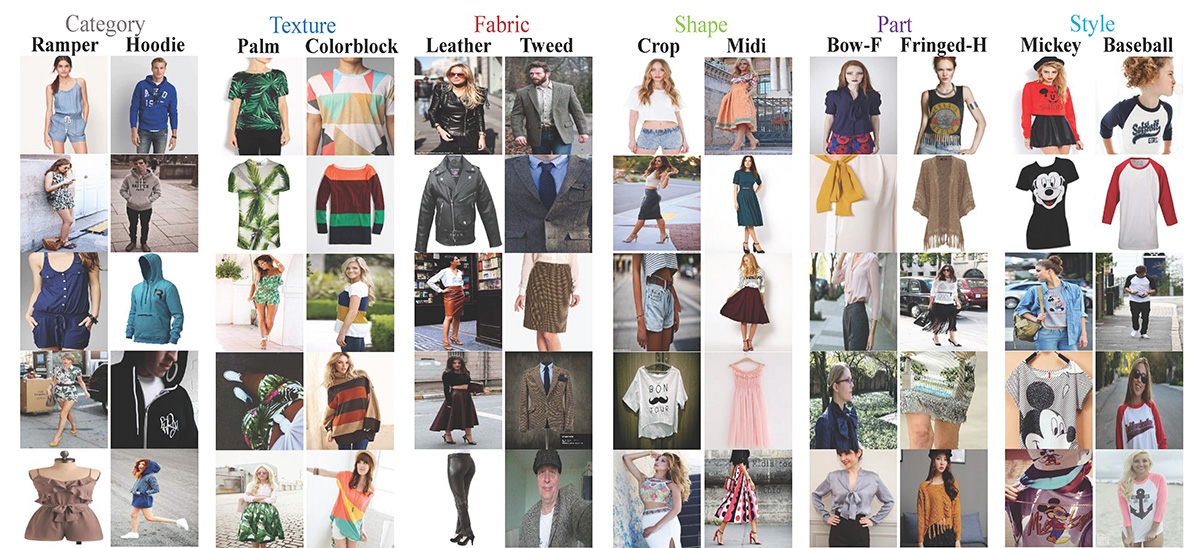
\includegraphics[totalheight=6cm]{imgs/img2.jpg}}
    \caption{Annotated Image}
    \label{fig:dataset}
\end{figure}

\subsection{Evaluation metric}

A suitable evaluation metric for image ranking is the ``precision at top-k'' measure which is popular score used to evaluate information retrieval systems. Precision at top k is defined as the proportion of retrieved items in the top-k set that are relevant to the query. We consider a retrieved image to be relevant when it belongs to the same class as the query image. The expression for precision at top-k hence becomes :
\begin{equation}\label{eqn3}
P_{k} = \frac{\sum_{i=1}^{k} I_{y_i, c}}{k}
\end{equation}
\begin{equation}\label{eqn3}
P_{avg} = \frac{\sum_{i=1}^{n} P_{k_i}}{n}
\end{equation}
Where $P_k$ is precision at top k evaluated on one query sample, $I_{y_i}$ is an indicator function which is 1 only when $y_i$ which is the class of the $i^{th}$ retrieved sample is same as $c$ which is the class of the query image. $P_{avg}$ is the top-k precision averaged over the complete dataset.

\begin{figure}[tph!]
\centerline{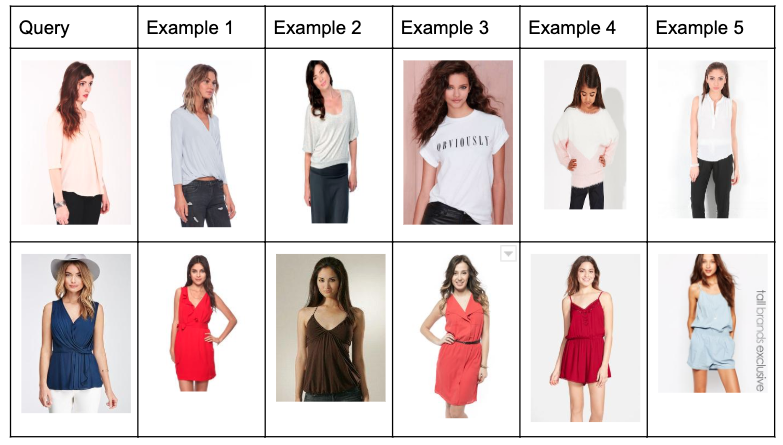
\includegraphics[totalheight=6cm]{imgs/top_5.png}}
    \caption{Top 5 best matches with respect to query image}
    \label{fig:top5}
\end{figure}

\begin{figure}[tph!]
\centerline{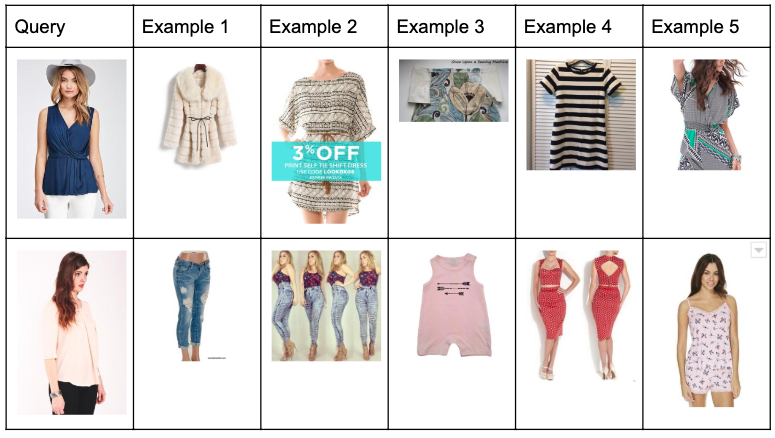
\includegraphics[totalheight=6cm]{imgs/Bottom_5.png}}
    \caption{Bottom 5 worst matches with respect to query image}
    \label{fig:Bottom_5}
\end{figure}